\documentclass{../base/base}
% Dateikodierung ist utf8
\usepackage[utf8]{inputenc}
\usepackage{url}
\usepackage[export]{adjustbox}
\usepackage{amsmath}
\usepackage{listings}
\usepackage{tikz}
\usepackage{tabularx}
\usepackage{color,colortbl}
\usepackage{ulem}
\usepackage{pdfpages}
\usepackage{ wasysym }
\usepackage{ booktabs }
\usepackage{lscape}
\usepackage{multicol}

\begin{document}

\Abgabeblatt{Assignment 3}{07.05.2018}{????}{????}{Yannis Rohloff (yannis@uni-bremen.de)}{Liu Meng(lium@uni-bremen.de)}{Peter Tschubij (tschupet@uni-bremen.de)}

\lstset{
    language=Python,
    basicstyle=\ttfamily\small,
    aboveskip={1.0\baselineskip},
    belowskip={1.0\baselineskip},
    columns=fixed,
    extendedchars=true,
    breaklines=true,
    tabsize=4,
    prebreak=\raisebox{0ex}[0ex][0ex]{\ensuremath{\hookleftarrow}},
    frame=lines,
    showtabs=false,
    showspaces=false,
    showstringspaces=false,
    keywordstyle=\color[rgb]{0.627,0.126,0.941},
    commentstyle=\color[rgb]{0.133,0.545,0.133},
    stringstyle=\color[rgb]{01,0,0},
    numbers=left,
    numberstyle=\small,
    stepnumber=1,
    numbersep=10pt,
    captionpos=t,
    escapeinside={\%*}{*)}
}


\section*{Exercise 1: Cutting Fabric - Variable Definition}

We definie our variable in a similar vein as any other coloring problem. Though it gets more complicated because shapes set constraints to neighboring parts.


Let's clarify a few terms. The \textit{workspace} is rectanglar arrangement of \textit{fields}. Each \textit{fields} should be filled by one \textit{tile}, where each \textit{tile} is a part of a shape.

We consider every field on our workspace to be uniquely identified by a coordinate tuple $c = (x,y)$, and the total field is a matrix $X'=[m_{x,y}]$.
\[
X'=
\begin{bmatrix}
    m_{11}       & m_{12} & m_{13} & \dots & m_{1w} \\
    m_{21}       & m_{22} & m_{23} & \dots & m_{2w} \\
    \hdotsfor{5} \\
    m_{h1}       & m_{h2} & m_{h3} & \dots & m_{hw}
\end{bmatrix}
\]
Every such field may only be occupied by one tile at a time, so that nothing overlaps. Furthermore every tile should be occupied by one tile with the exception of continouus patterns at the beginning and the end of a workspace.

A tile is represented by a 3-tuple $t = (s, r, n)$ where $m$ is the number its the shape from the input, $r$ is a number from $1$ to $4$ representing the rotation. and $n$ is the number of the tile of the shape.
We will copy every shape from the input four times to where each time w increase the $r$ accordingly.
Let $T$ be the set of all these $tiles$.
%--------------------------------------------------------------------------
\begin{comment}

Now we can define a Variable stating if a field is occupied by a tile:
$$X_{c,s} = X_{(x,y),(s,r,n)}$$

To formulate all constraints we need to extend the workspace form the excersise. The input is a workspace of dimensions $w \cdot h$, with $h$ beeing the axis that can extend and w the width. No tile may be placed outside of the width.

First, we copy another workspace directly beneath the current workspace. This results in the height to double: $h := h \cdot 2$
Let $F2$ be the set of the added fields, while $F1$ is the set of fields that existeed before. And let $F = F1 \cup F2$

Second, we add another column on each side. The new width is $h := h+2$. We will use these fields to ensure that they are not \textit{painted} with e tile. Let $O$ be the set of these fields.

With $h=3,w=2$ the field looks like this. The blue fields are in $O$, the yellow fields are in $F1$ and the orange fields are $F2$ \\

\end{comment}
%--------------------------------------------------------------------------

Now we expand the workspace matrix into $ (2h-1)*w $, namely $X=[m_{x,y}]$, $\substack{x \in \{1,...,2h-1\}}$.
\[
X=
\begin{bmatrix}
    m_{11}       & m_{12} & m_{13} & \dots & m_{1w} \\
    m_{21}       & m_{22} & m_{23} & \dots & m_{2w} \\
    \hdotsfor{5} \\
    m_{(2h-1) 1}       & m_{(2h-1) 2} & m_{(2h-1) 3} & \dots & m_{(2h-1) w}
\end{bmatrix}
\]
For example, when $h=3$, $w=4$, the new workspace looks like (yellow parts are the expanded part):
\begin{center}
    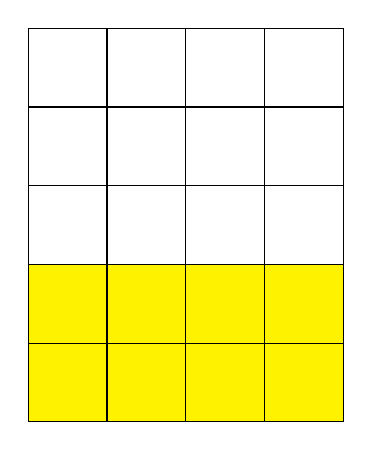
\begin{tikzpicture}[scale=1]
    \draw [fill=yellow] (0,1) rectangle (1,2);
    \draw [fill=yellow] (1,1) rectangle (2,2);
    \draw [fill=yellow] (2,1) rectangle (3,2);
    \draw [fill=yellow] (3,1) rectangle (4,2);

    \draw [fill=yellow] (0,2) rectangle (1,3);
    \draw [fill=yellow] (1,2) rectangle (2,3);
    \draw [fill=yellow] (2,2) rectangle (3,3);
    \draw [fill=yellow] (3,2) rectangle (4,3);

    \draw [fill=white] (0,3) rectangle (1,4);:
    \draw [fill=white] (1,3) rectangle (2,4);
    \draw [fill=white] (2,3) rectangle (3,4);
    \draw [fill=white] (3,3) rectangle (4,4);

    \draw [fill=white] (0,4) rectangle (1,5);
    \draw [fill=white] (1,4) rectangle (2,5);
    \draw [fill=white] (2,4) rectangle (3,5);
    \draw [fill=white] (3,4) rectangle (4,5);

    \draw [fill=white] (0,5) rectangle (1,6);
    \draw [fill=white] (1,5) rectangle (2,6);
    \draw [fill=white] (2,5) rectangle (3,6);
    \draw [fill=white] (3,5) rectangle (4,6);
    \end{tikzpicture} 
\end{center}
Then we add the first constraint.
\subsection{Constraint 1: every column in the new workspace should have $h$ tiles}
$$\bigwedge_{y \in \{1,..w\}, b=h} m_{y,b}$$
$b$ means block(tile)
Then the workspace may looks like following (orange parts are tiles):
\begin{center}    
    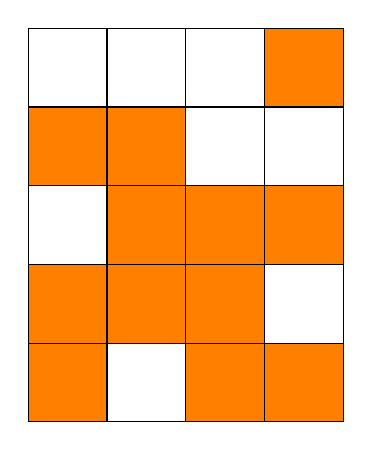
\begin{tikzpicture}[scale=1]
    \draw [fill=orange] (0,1) rectangle (1,2);
    \draw [fill=white] (1,1) rectangle (2,2);
    \draw [fill=orange] (2,1) rectangle (3,2);
    \draw [fill=orange] (3,1) rectangle (4,2);

    \draw [fill=orange] (0,2) rectangle (1,3);
    \draw [fill=orange] (1,2) rectangle (2,3);
    \draw [fill=orange] (2,2) rectangle (3,3);
    \draw [fill=white] (3,2) rectangle (4,3);

    \draw [fill=white] (0,3) rectangle (1,4);:
    \draw [fill=orange] (1,3) rectangle (2,4);
    \draw [fill=orange] (2,3) rectangle (3,4);
    \draw [fill=orange] (3,3) rectangle (4,4);

    \draw [fill=orange] (0,4) rectangle (1,5);
    \draw [fill=orange] (1,4) rectangle (2,5);
    \draw [fill=white] (2,4) rectangle (3,5);
    \draw [fill=white] (3,4) rectangle (4,5);

    \draw [fill=white] (0,5) rectangle (1,6);
    \draw [fill=white] (1,5) rectangle (2,6);
    \draw [fill=white] (2,5) rectangle (3,6);
    \draw [fill=orange] (3,5) rectangle (4,6);
    \end{tikzpicture}
\end{center}

\subsection{Constraint 2: every column in the new workspace should have $h$ continual tiles}
$$\bigwedge_{y \in \{1,..w\}, \substack{c \in \{0,1\}}} m_{y,c}$$
Then the workspace looks like following:
\begin{center}    
    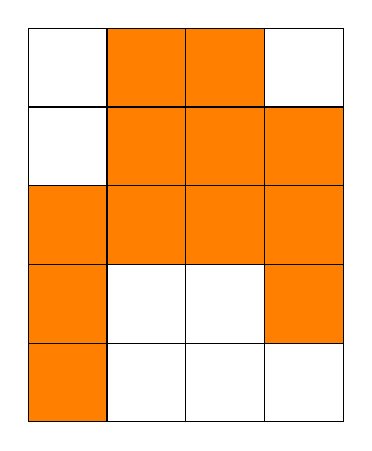
\begin{tikzpicture}[scale=1]
    \draw [fill=orange] (0,1) rectangle (1,2);
    \draw [fill=white] (1,1) rectangle (2,2);
    \draw [fill=white] (2,1) rectangle (3,2);
    \draw [fill=white] (3,1) rectangle (4,2);

    \draw [fill=orange] (0,2) rectangle (1,3);
    \draw [fill=white] (1,2) rectangle (2,3);
    \draw [fill=white] (2,2) rectangle (3,3);
    \draw [fill=orange] (3,2) rectangle (4,3);

    \draw [fill=orange] (0,3) rectangle (1,4);:
    \draw [fill=orange] (1,3) rectangle (2,4);
    \draw [fill=orange] (2,3) rectangle (3,4);
    \draw [fill=orange] (3,3) rectangle (4,4);

    \draw [fill=white] (0,4) rectangle (1,5);
    \draw [fill=orange] (1,4) rectangle (2,5);
    \draw [fill=orange] (2,4) rectangle (3,5);
    \draw [fill=orange] (3,4) rectangle (4,5);

    \draw [fill=white] (0,5) rectangle (1,6);
    \draw [fill=orange] (1,5) rectangle (2,6);
    \draw [fill=orange] (2,5) rectangle (3,6);
    \draw [fill=white] (3,5) rectangle (4,6);
    \end{tikzpicture}
\end{center}
%--------------------------------------------------------------------------
\begin{comment}
\textbf{Further explanation why copying the workspace once is suficcient follows\dots}

Now we can define constraints that define our problem. Some are similar thoses of the Graph Coloring Problem, since essentially we paint each field with a tile. 


\subsection{Constraint 1: No border has a tile.}
$$\bigwedge_{\substack{c \in O}} \bigwedge_{\substack{t \in T}} \neg X_{c,t}$$

\subsection{Constraint 2: Every field in F1 and F2 has at least one tile}
$$\bigwedge_{\substack{c \in F}} \bigvee_{\substack{t \in T }} X_{c,t}$$


\subsection{Constraint 3: Every field in F1 and F2 has at most one tile.}
$$\bigwedge_{\substack{c \in F}} \bigvee_{\substack{t1,t1 \in T \\ t1 \neq t2 }} \neg X_{c,t1} \lor \neg X_{c,t2}$$

\subsection{Constraint 4: Respective fields in and F1 and F2 have the same tiles assigned}
$$\bigwedge_{\substack{(x,y) \in F1}} \bigvee_{\substack{t \in T}} \neg X_{(x,y),t} \lor X_{(x,y+h),t} $$
and
$$\bigwedge_{\substack{(x,y) \in F1}} \bigvee_{\substack{t \in T}} \neg X_{(x,y+h),t} \lor X_{(x,y),t} $$
(Note that you can read both as implications. Since we have both directions the implications are bidirectional)


\subsection{Constraint 5: If a tile is connected on a field, the neighbors of the field are filled with the neighbors of the tile in the shape.}

We define the sets $V$ and $H$ containing tuples of all the vertical connections and horizontal connections. (Only top to bottom and left to right. They are not bidirectional)
For example: $((t1,t2) \in V$ if We have the shape:\\
.+\\
.+\\
(Note: we rotated the file shape four times so actually we have two tuples in H and two in V)\\

Horizontal:
$$\bigwedge_{\substack{(x,y) \in F\cup O}}\ \  \bigwedge_{\substack{(t1,t2) \in H}} \neg X_{(x,y),t1} \lor X_{(x+1,y),t2} $$
Horizontal back implication:
$$\bigwedge_{\substack{(x,y) \in F\cup O}}\ \  \bigwedge_{\substack{(t1,t2) \in H}} X_{(x,y),t1} \lor \neg X_{(x+1,y),t2} $$

Vertical:
$$\bigwedge_{\substack{(x,y) \in F\cup O}}\ \  \bigwedge_{\substack{(t1,t2) \in V}} \neg  X_{(x,y),t1} \lor X_{(x,y+1),t2} $$
Vertical back implication:
$$\bigwedge_{\substack{(x,y) \in F\cup O}}\ \  \bigwedge_{\substack{(t1,t2) \in V}} X_{(x,y),t1} \lor \neg X_{(x,y+1),t2} $$


\end{comment}
%--------------------------------------------------------------------------


\end{document}
